% fl-iot-ids: Federated Learning-Based Intrusion Detection for Distributed IoT Networks
% Nyiko Mathebula, EEE4022S final-year project, University of Cape Town, 2026
%
% Figure 4.2: one federated round (FedAvg and FedProx), in the style of Figures 3.1 and 4.1.
% Run from the project root (needs lualatex):
%   lualatex -output-directory=results/report/figures src/report/diagrams/fig4_2_federated_round.tex
%   pdftoppm -r 300 -png -singlefile results/report/figures/fig4_2_federated_round.pdf results/report/figures/ch4_2_federated_round
% Edit the words inside the \node[...] {...} commands below to change a label.
\documentclass[border=6pt]{standalone}
\usepackage{fontspec}
\IfFontExistsTF{Inter}{\setmainfont{Inter}}{\setmainfont{DejaVu Sans}}
\usepackage{amsmath}
\usepackage{unicode-math}
\setmathfont{Latin Modern Math}
\usepackage{tikz}
\usetikzlibrary{arrows.meta,positioning,fit,backgrounds,calc}

\definecolor{ink}{HTML}{1D2230}
\definecolor{sub}{HTML}{454B5C}
\definecolor{arrowc}{HTML}{3A3F4B}
\definecolor{procF}{HTML}{F2F3FD}\definecolor{procS}{HTML}{9097C4}
\definecolor{modelF}{HTML}{CFE1FB}\definecolor{modelS}{HTML}{5B8FD6}
\definecolor{storeF}{HTML}{CDF3FB}\definecolor{storeS}{HTML}{38A8C2}
\definecolor{endF}{HTML}{36B6F2}\definecolor{endS}{HTML}{1A86C2}

\begin{document}
\thickmuskip=5mu \medmuskip=4mu \thinmuskip=3mu
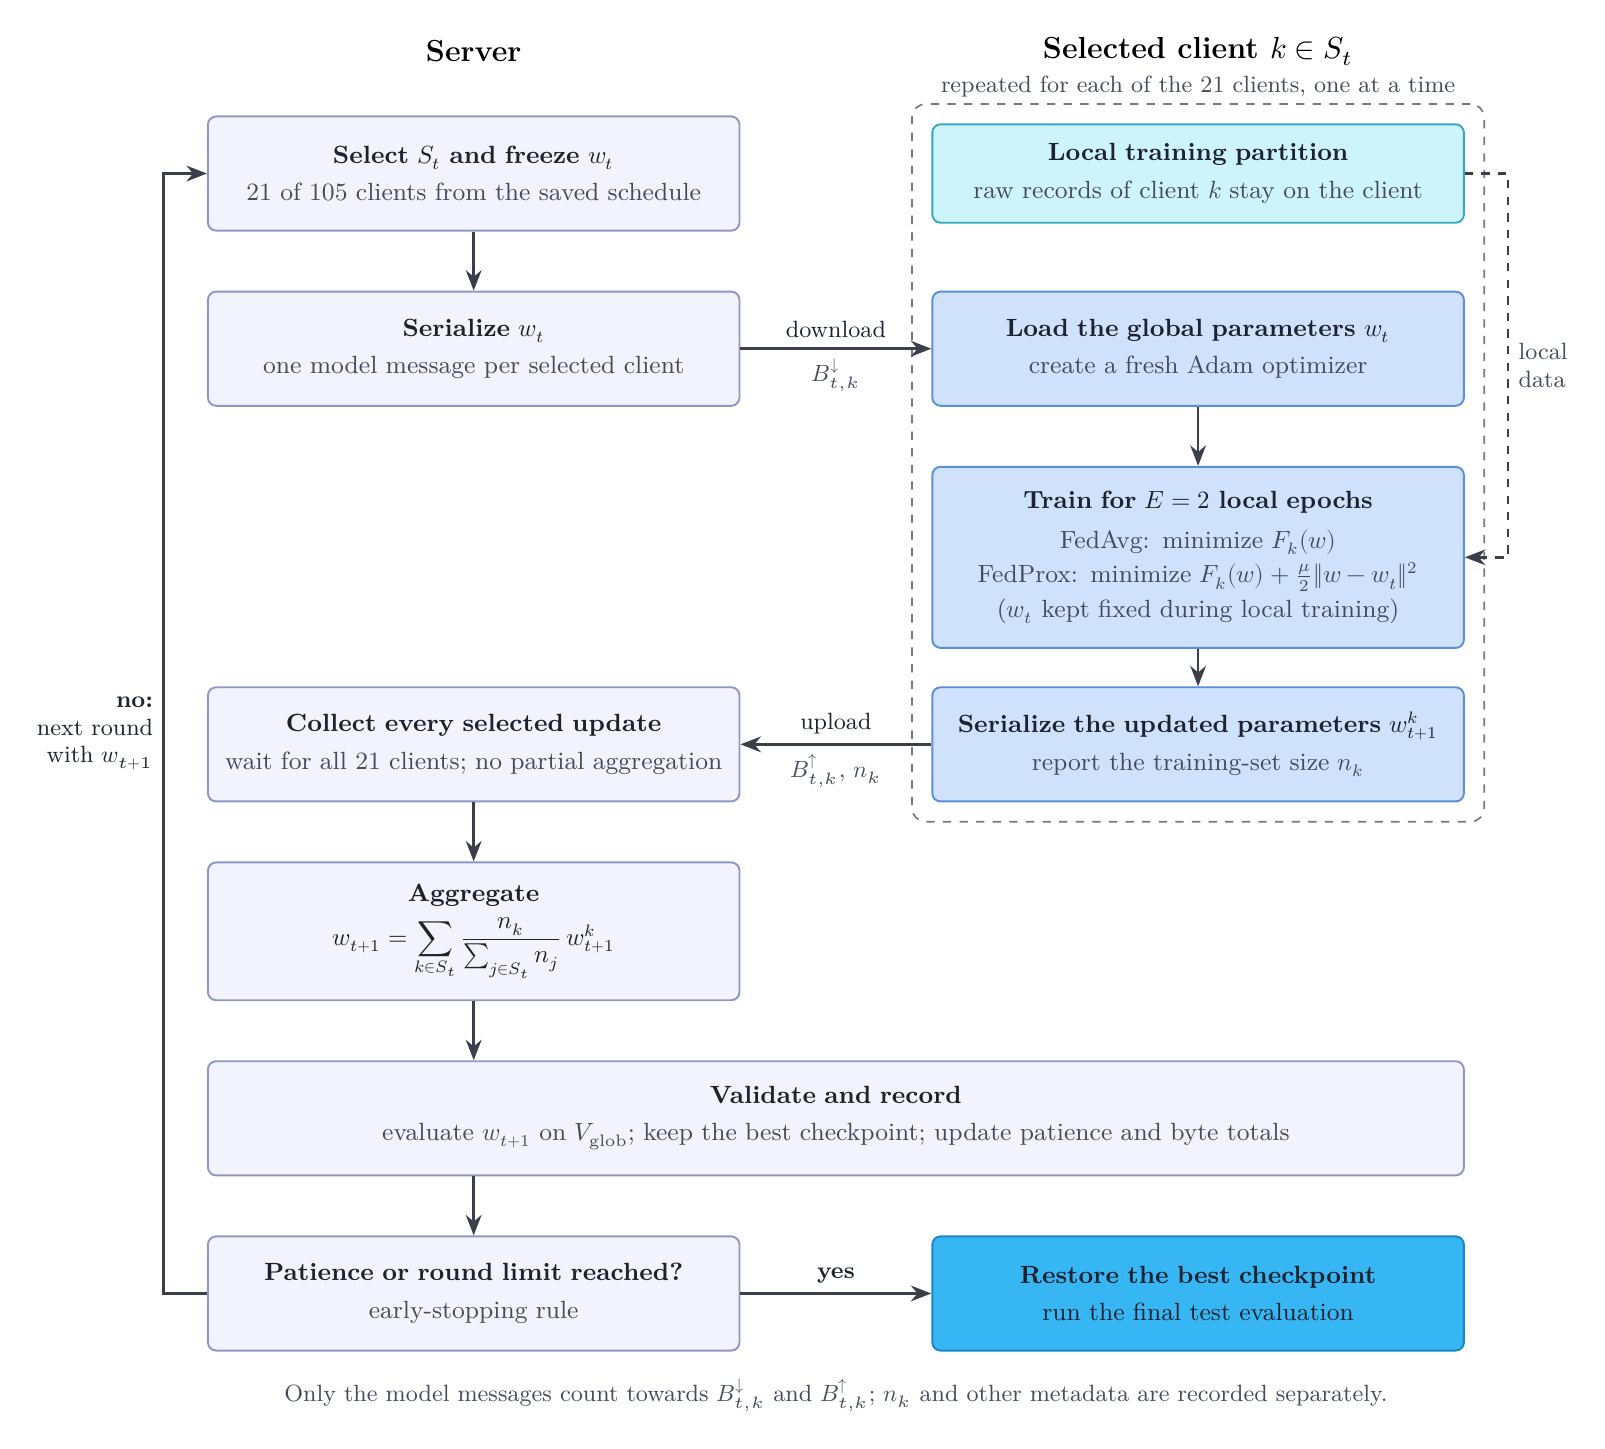
\begin{tikzpicture}[
  font=\fontsize{9}{11.5}\selectfont, >={Stealth[length=2.6mm,width=2mm]},
  base/.style={execute at begin node={\thickmuskip=5mu \medmuskip=4mu}, rounded corners=3pt, line width=0.7pt, align=center, inner sep=5pt, text=ink},
  server/.style={base, draw=procS, fill=procF, text width=6.4cm, minimum height=1.45cm},
  client/.style={base, draw=modelS, fill=modelF, text width=6.4cm, minimum height=1.45cm},
  store/.style={base, draw=storeS, fill=storeF, text width=6.4cm, minimum height=1.25cm},
  final/.style={base, draw=endS, fill=endF, text width=6.4cm, minimum height=1.45cm},
  arr/.style={->, draw=arrowc, line width=0.9pt},
  lab/.style={font=\fontsize{8.5}{10}\selectfont, text=sub},
  t/.style={font=\bfseries\fontsize{10}{12}\selectfont},
]
% ------------------------------------------------------------- column headers
\node[t, font=\bfseries\fontsize{11}{13}\selectfont] (hs) at (0, 1.55) {Server};
\node[t, font=\bfseries\fontsize{11}{13}\selectfont] (hc) at (9.2, 1.55) {Selected client $k\in S_t$};
\node[lab] at (9.2, 1.1) {repeated for each of the 21 clients, one at a time};

% ------------------------------------------------------------- server column
\node[server] (s1) at (0, 0) {{\bfseries Select $S_t$ and freeze $w_t$}\\[2pt]
  {\color{sub} 21 of 105 clients from the saved schedule}};
\node[server, below=0.75cm of s1] (s2) {{\bfseries Serialize $w_t$}\\[2pt]
  {\color{sub} one model message per selected client}};
\node[server, below=3.55cm of s2] (s3) {{\bfseries Collect every selected update}\\[2pt]
  {\color{sub} wait for all 21 clients; no partial aggregation}};
\node[server, below=0.75cm of s3, minimum height=1.75cm] (s4) {{\bfseries Aggregate}\\[3pt]
  $\displaystyle w_{t+1}=\sum_{k\in S_t}\frac{n_k}{\sum_{j\in S_t}n_j}\,w^{k}_{t+1}$};

% ------------------------------------------------------------- client column
\node[store] (c0) at (9.2, 0) {{\bfseries Local training partition}\\[2pt]
  {\color{sub} raw records of client $k$ stay on the client}};
\node[client] (c1) at (c0 |- s2) {{\bfseries Load the global parameters $w_t$}\\[2pt]
  {\color{sub} create a fresh Adam optimizer}};
\node[client, below=0.75cm of c1, minimum height=2.3cm] (c2) {{\bfseries Train for $E=2$ local epochs}\\[3pt]
  {\color{sub}FedAvg: minimize $F_k(w)$}\\[1pt]
  {\color{sub}FedProx: minimize $F_k(w)+\frac{\mu}{2}\lVert w-w_t\rVert^2$}\\[1pt]
  {\color{sub}($w_t$ kept fixed during local training)}};
\node[client] (c3) at (c0 |- s3) {{\bfseries Serialize the updated parameters $w^{k}_{t+1}$}\\[2pt]
  {\color{sub} report the training-set size $n_k$}};

% client group frame
\begin{scope}[on background layer]
  \node[draw=arrowc!70, dashed, rounded corners=5pt, line width=0.6pt, inner sep=7pt,
        fit=(c0)(c3)] (grp) {};
\end{scope}

% ------------------------------------------------------------- full-width steps
\node[server, text width=15.6cm, below=0.75cm of s4.south west, anchor=north west] (s5)
  {{\bfseries Validate and record}\\[2pt]
   {\color{sub} evaluate $w_{t+1}$ on $V_{\mathrm{glob}}$; keep the best checkpoint; update patience and byte totals}};
\node[server, text width=6.4cm, below=0.75cm of s5.south west, anchor=north west] (s6)
  {{\bfseries Patience or round limit reached?}\\[2pt]
   {\color{sub} early-stopping rule}};
\node[final, anchor=west] (s7) at (s6.east -| c3.west) {{\bfseries Restore the best checkpoint}\\[2pt]
  run the final test evaluation};

% ------------------------------------------------------------- arrows
\draw[arr] (s1) -- (s2);
\draw[arr] (s2.east) -- node[above, lab, text=ink]{download} node[below, lab]{$B^{\downarrow}_{t,k}$} (c1.west);
\draw[arr] (c1) -- (c2);
\draw[arr] (c2) -- (c3);
\draw[arr] (c3.west) -- node[above, lab, text=ink]{upload} node[below, lab]{$B^{\uparrow}_{t,k}$, $n_k$} (s3.east);
\draw[arr, dashed] (c0.east) -- ++(0.55,0) |- node[pos=0.25, right, lab, align=left]{local\\data} (c2.east);
\draw[arr] (s3) -- (s4);
\draw[arr] (s4) -- (s4 |- s5.north);
\draw[arr] (s5.south -| s6) -- (s6);
\draw[arr] (s6.east) -- node[above, lab, text=ink]{\bfseries yes} (s7.west);
\draw[arr] (s6.west) -- ++(-0.55,0) |- node[pos=0.25, left, lab, text=ink, align=right]{\bfseries no:\\next round\\with $w_{t+1}$} (s1.west);

% ------------------------------------------------------------- note
\node[lab, anchor=north] at ($(s5.south)+(0,-2.45)$)
  {Only the model messages count towards $B^{\downarrow}_{t,k}$ and $B^{\uparrow}_{t,k}$; $n_k$ and other metadata are recorded separately.};
\end{tikzpicture}
\end{document}
